\documentclass{sig-alternate-ipsn13}
\usepackage{graphicx}

\begin{document}

\title{WiP Abstract: Preliminary Evaluation of ROS2}
% Format\titlenote{(Does NOT produce the permission block, copyright information nor page numbering). Supported by ACM.}}
%
% You need the command \numberofauthors to handle the 'placement
% and alignment' of the authors beneath the title.
%
% For aesthetic reasons, we recommend 'three authors at a time'
% i.e. three 'name/affiliation blocks' be placed beneRath the title.
%
% NOTE: You are NOT restricted in how many 'rows' of
% "name/affiliations" may appear. We just ask that you restrict
% the number of 'columns' to three.
%
% Because of the available 'opening page real-estate'
% we ask you to refrain from putting more than six authors
% (two rows with three columns) beneath the article title.
% More than six makes the first-page appear very cluttered indeed.
%
% Use the \alignauthor commands to handle the names
% and affiliations for an 'aesthetic maximum' of six authors.
% Add names, affiliations, addresses for
% the seventh etc. author(s) as the argument for the
% \additionalauthors command.
% These 'additional authors' will be output/set for you
% without further effort on your part as the last section in
% the body of your article BEFORE References or any Appendices.

\numberofauthors{3} %  in this sample file, there are a *total*
% of EIGHT authors. SIX appear on the 'first-page' (for formatting
% reasons) and the remaining two appear in the \additionalauthors section.
%
\author{
% You can go ahead and credit any number of authors here,
% e.g. one 'row of three' or two rows (consisting of one row of three
% and a second row of one, two or three).
%
% The command \alignauthor (no curly braces needed) should
% precede each author name, affiliation/snail-mail address and
% e-mail address. Additionally, tag each line of
% affiliation/address with \affaddr, and tag the
% e-mail address with \email.
%
% 1st. author
\alignauthor Yuya Maruyama\\
\affaddr{School of Engineering Science}\\
\affaddr{Osaka University}\\
       % \affaddr{Institute for Clarity in Documentation}\\
       % \affaddr{1932 Wallamaloo Lane}\\
       % \affaddr{Wallamaloo, New Zealand}\\
       % \email{trovato@corporation.com}
% 2nd. author
\alignauthor Shinpei Kato\\
\affaddr{Graduate School of Information Science}\\
\affaddr{Nagoya University}\\
       % \affaddr{Institute for Clarity in Documentation}\\
       % \affaddr{P.O. Box 1212}\\
       % \affaddr{Dublin, Ohio 43017-6221}\\
       % \email{webmaster@marysville-ohio.com}
% 3rd. author
\alignauthor Takuya Azumi\\
\affaddr{Graduate School of Engineering Science}\\
\affaddr{Osaka University}\\
       % \affaddr{The Th{\o}rv{\"a}ld Group}\\
       % \affaddr{1 Th{\o}rv{\"a}ld Circle}\\
       % \affaddr{Hekla, Iceland}\\
       % \email{larst@affiliation.org}
% \and  % use '\and' if you need 'another row' of author names
% % 4th. author
% \alignauthor Lawrence P. Leipuner\\
%        \affaddr{Brookhaven Laboratories}\\
%        \affaddr{Brookhaven National Lab}\\
%        \affaddr{P.O. Box 5000}\\
%        \email{lleipuner@researchlabs.org}
% % 5th. author
% \alignauthor Sean Fogarty\\
%        \affaddr{NASA Ames Research Center}\\
%        \affaddr{Moffett Field}\\
%        \affaddr{California 94035}\\
%        \email{fogartys@amesres.org}
% % 6th. author
% \alignauthor Charles Palmer\\
%        \affaddr{Palmer Research Laboratories}\\
%        \affaddr{8600 Datapoint Drive}\\
%        \affaddr{San Antonio, Texas 78229}\\
%        \email{cpalmer@prl.com}
}
% There's nothing stopping you putting the seventh, eighth, etc.
% author on the opening page (as the 'third row') but we ask,
% for aesthetic reasons that you place these 'additional authors'
% in the \additional authors block, viz.
% \additionalauthors{Additional authors: John Smith (The Th{\o}rv{\"a}ld Group,
% email: {\texttt{jsmith@affiliation.org}}) and Julius P.~Kumquat
% (The Kumquat Consortium, email: {\texttt{jpkumquat@consortium.net}}).}
% \date{30 July 1999}
% Just remember to make sure that the TOTAL number of authors
% is the number that will appear on the first page PLUS the
% number that will appear in the \additionalauthors section.

\maketitle
% \begin{abstract}

% \end{abstract}

% \section{Introduction}

Cyber-Physical Systems (CPS) represent the next generation of distributed and embedded systems. CPS applications have become increasingly complicated and diverse to monitor and control complex real-time phenomena. The Robot Operating System (ROS), an open-source middleware for robotics development, has been widely used for CPS applications (e.g., autonomous cars). ROS provides publish/subscribe transport, multiple libraries (e.g., Point Cloud Library), and tools to help software developers create CPS applications.


However, ROS does not meet real-time run requirements and only runs on a few types of OSs. Therefore, ROS is not suitable for real-time, embedded systems. To address this problem, ROS will undergo a significant upgrade and will be known as ROS2 \cite{ros2_iccps2016}. ROS2 considers the following use cases: real-time systems, non-ideal networks, small embedded systems, and cross-platform.

The existing version of ROS (hereinafter referred to as ROS1) will be reconstructed with improving user interface APIs and utilize new technologies (e.g., Data Distribution Service (DDS) \cite{pardo2003omg}). The ROS1 transport system will be replaced by DDS, an industry-standard real-time communication system and end-to-end middleware that can provides reliable publish/subscribe transport.

The next-generation communication system of ROS2, DDS, is suitable for CPS due to its various transport configurations, such as DEADLINE, RELIABILITY, and DURABILITY. It has multiple implementations, including small/embedded solutions to reduce library sizes and memory footprints. Developed by different DDS vendors, several implementations have been used in mission-critical environments and have been verified by NASA. Therefore, ROS2, by using DDS, is reliable and flexible.

Figure \ref{fig:graph} shows the data communication time between nodes using ROS1 and ROS2. Using DDS, ROS2 has various transport configurations available that cause a certain amount of overhead. ROS2 needs to convert data for DDS and abstract DDS from ROS2 users. The overhead contains these transactions in addition to the difference between the ROS1 communication system and DDS. These influences vary depending on the transport situation, data size, and DDS vendor.

In this study, we clarify the performance characteristics of currently available data transport between nodes for ROS1 and ROS2 in various situations. Showcasing the present capability of ROS2, depending on DDS vendors and configurations, we explore and evaluate the constraints facing ROS2 and its potential. The advantages and disadvantages of ROS2 are clarified along with problems in the case where ROS1 and ROS2 coexist. To the best of our knowledge, this evaluation is the first to explore the ROS2's performance.

% \begin{figure}[t]
% \begin{center}
% \includegraphics{fly.eps}
% \caption{A sample black and white graphic (.eps format).}
% \label{fig:example}
% \end{figure}

% \begin{figure}[t]
% \begin{center}
% 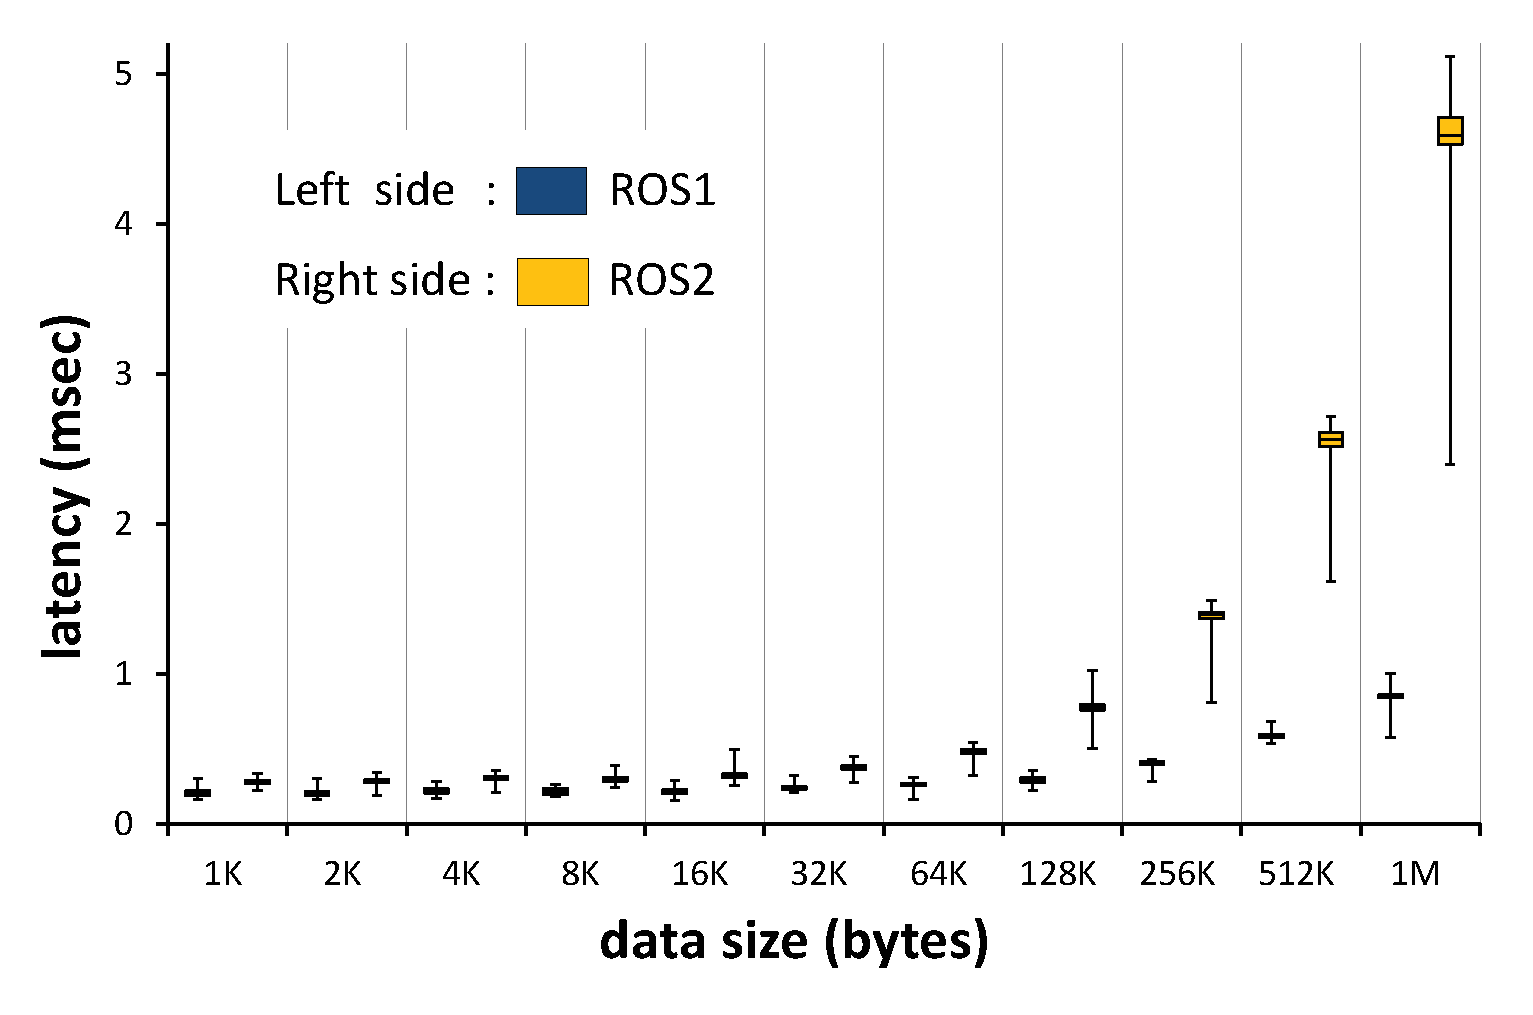
\includegraphics{graph.eps}
% \caption{A sample black and white graphic (.eps format).}
% \label{fig:example}
% \end{figure}

\begin{figure}[t]
\begin{center}
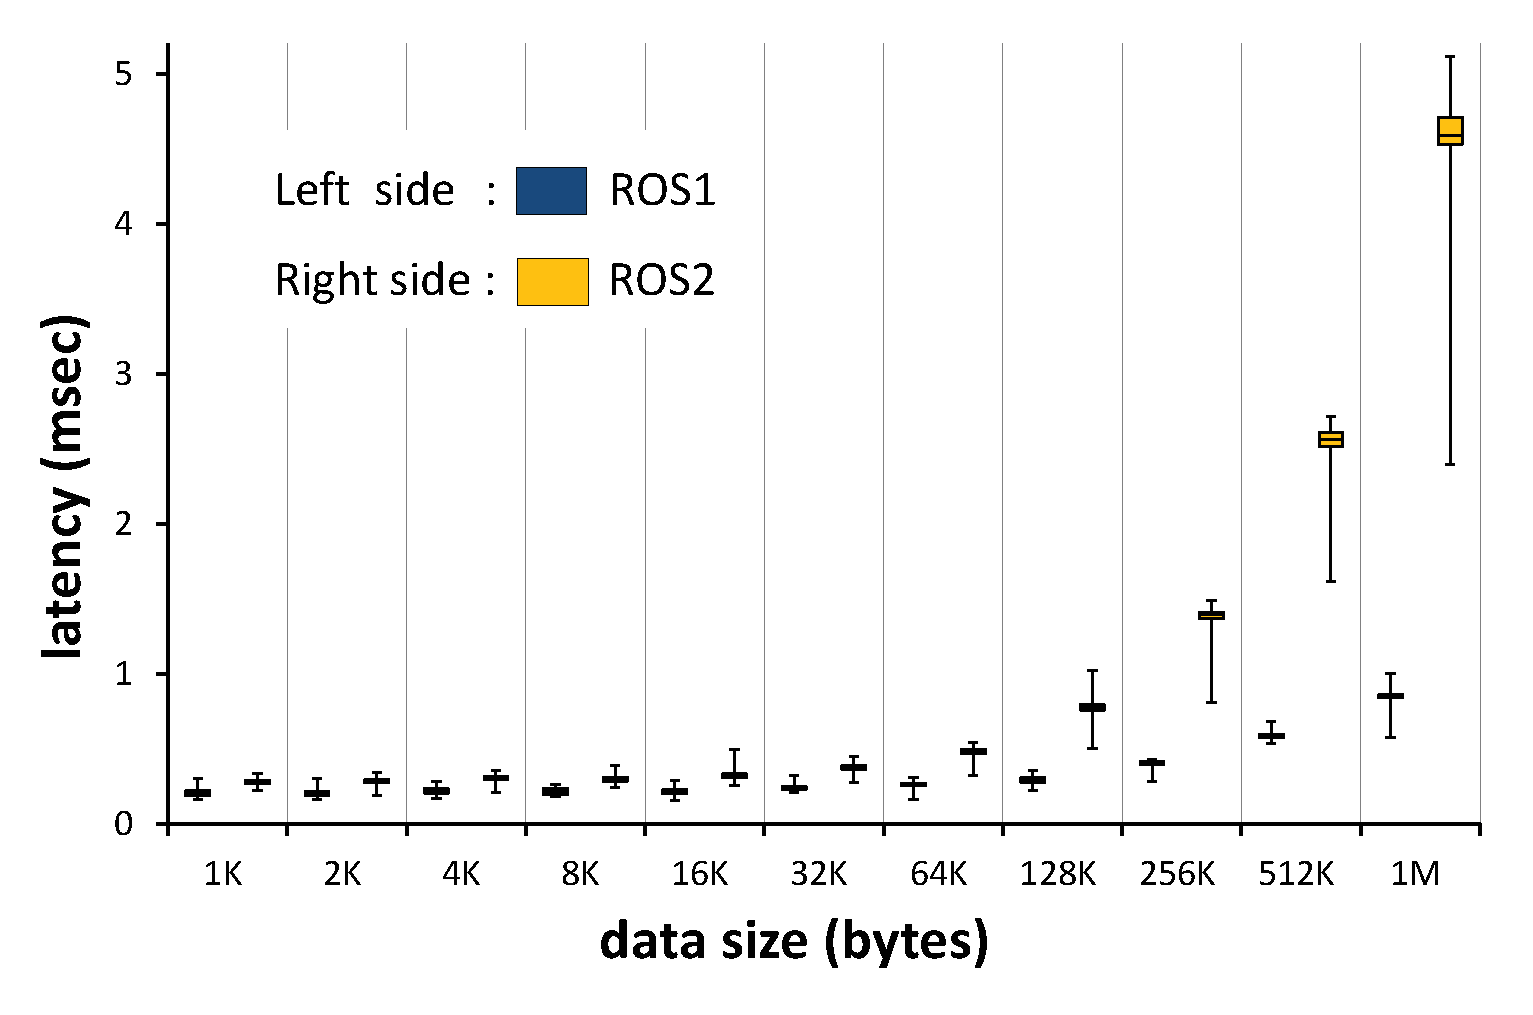
\includegraphics[scale=0.33]{graph.eps}
%\epsfig{file=sys_config_2.eps, width=80mm}
\end{center}
\vspace{-8.mm}
\caption{Comparison of the transport latency variation versus data size for ROS1 and ROS2.}
\vspace{-5.0mm}
\label{fig:graph}
\end{figure}

% \section{Conclusions}
% Conclusion goes here.

%ACKNOWLEDGMENTS are optional
% \section*{Acknowledgments}
% Acknowledgement goes here.

%
% The following two commands are all you need in the
% initial runs of your .tex file to
% produce the bibliography for the citations in your paper.
% \bibliography{sigproc}  % sigproc.bib is the name of the Bibliography in this case
\vspace{-3.0mm}
\bibliographystyle{abbrv}
\bibliography{reference}

% You must have a proper ".bib" file
%  and remember to run:
% latex bibtex latex latex
% to resolve all references
%
% ACM needs 'a single self-contained file'!
%
%APPENDICES are optional
%\balancecolumns
% \appendix
% %Appendix A

% Appendix goes here.

% That's all folks!
\end{document}
